\appendix
\renewcommand{\thesection}{A.\arabic{section}}
\renewcommand{\thesubsection}{A.\arabic{section}.\arabic{subsection}}
\renewcommand{\thesubsubsection}{A.\arabic{section}.\arabic{subsection}.\arabic{subsubsection}}
\renewcommand\thefigure{A.\arabic{section}.\arabic{figure}}   
\renewcommand\thetable{A.\arabic{section}.\arabic{table}}  
\renewcommand\thecode{A.\arabic{section}.\arabic{code}}  
\appendixpage
\addappheadtotoc
\section{Glosario y abreviaciones}
\printglossary
\printglossary[type=\acronymtype, title=Abreviaciones]
\afterpage{\blankpage}
\newpage
\section{Formularios}
\begin{figure}[H]
	\caption{Formulario de  registro de movimiento (blanco)}
	\label{fig:frmWhiteMov}
	\centering
	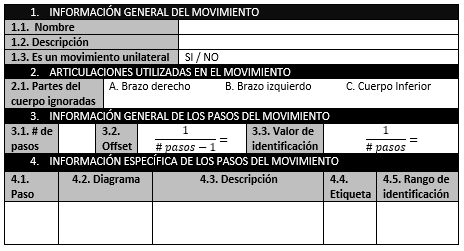
\includegraphics[width=430px,height=200px]{graphics/frm-movimiento.PNG} \\
	\textbf{Fuente:} Elaborado por el autor de tesis
\end{figure}

\begin{figure}[H]
	\caption{Formulario de  registro de rutina (blanco)}
	\label{fig:frmWhiteRout}
	\centering
	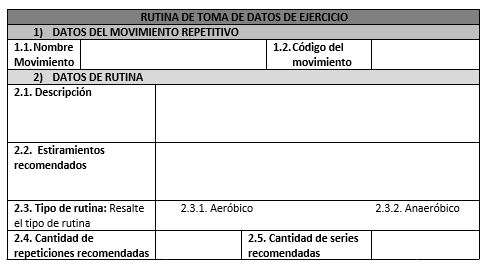
\includegraphics[width=430px,height=230px]{graphics/frm-rutina.PNG} \\
	\textbf{Fuente:} Elaborado por el autor de tesis
\end{figure}
\section{Ejercicios para calentamientos} \label{anx:warmup}
\begin{figure}[H]
	\caption{Ejercicios de calentamientos 1}
	\label{fig:anxWarmup1}
	\centering
	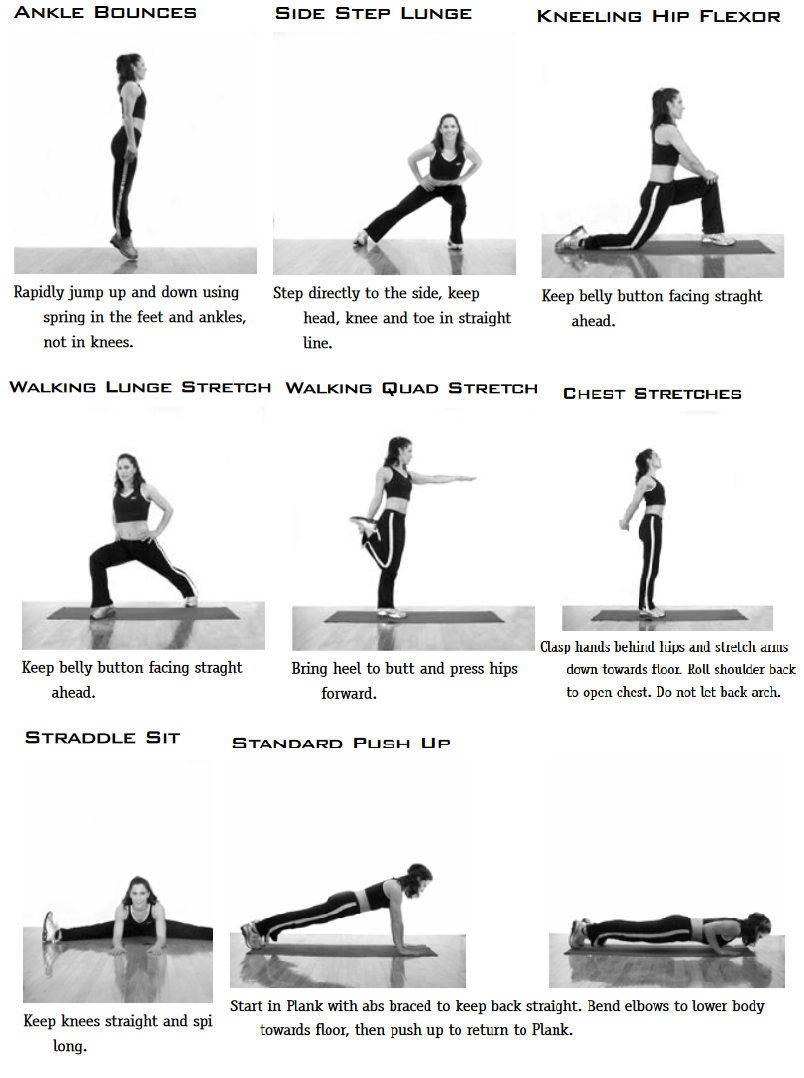
\includegraphics[width=430px,height=580px]{graphics/warmup1.PNG} \\
	\textbf{Fuente:} \cite{arbour2006strength}
\end{figure}

\begin{figure}[H]
	\caption{Ejercicios de calentamientos 2}
	\label{fig:anxWarmup2}
	\centering
	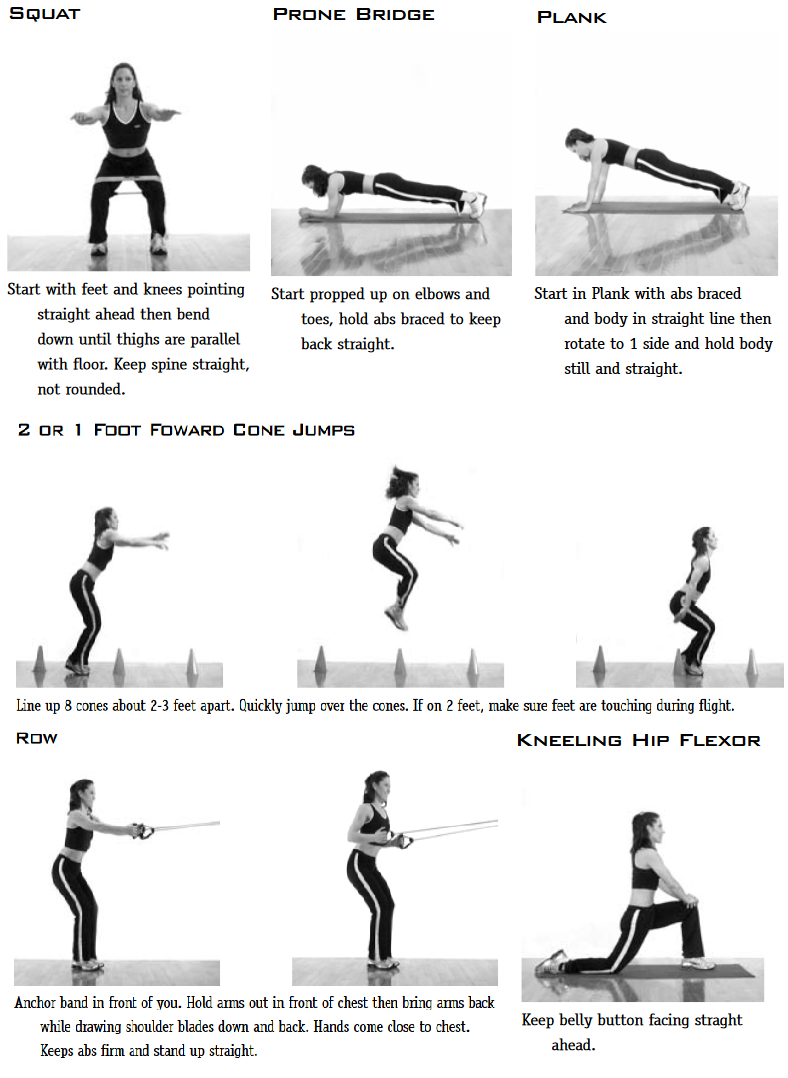
\includegraphics[width=430px,height=600px]{graphics/warmup2.PNG} \\
	\textbf{Fuente:} \cite{arbour2006strength}
\end{figure}

\begin{figure}[H]
	\caption{Ejercicios de calentamientos 3}
	\label{fig:anxWarmup3}
	\centering
	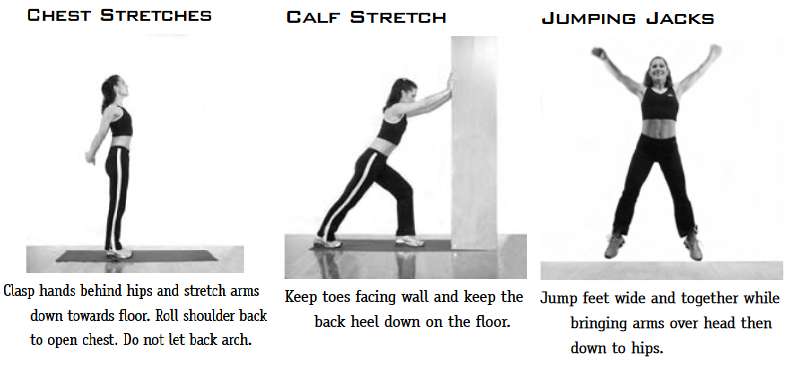
\includegraphics[width=430px,height=180px]{graphics/warmup3.PNG} \\
	\textbf{Fuente:} \cite{arbour2006strength}
\end{figure}

\section{Hojas de observaciones}
\begin{table}[H]
\begin{center}
\caption{Ejemplo de observaciones de datos de profundidades entre el usuario y el Kinect}
\label{tab:obsDepth}
\begin{tabular}{|l|l|l|}
\hline
Joint & Altura & Profundidad \\ \hline
0 & 1,55724901 & 3,523197651 \\ \hline
0 & 1,14456409 & 3,611632586 \\ \hline
0 & 1,33391045 & 3,508765697 \\ \hline
\multicolumn{3}{l}{\textbf{Fuente:} Elaborado por el autor de tesis}
\end{tabular}
\end{center}
\end{table}

\begin{table}[H]
\begin{center}
\caption{Ejemplo de observaciones de los errores del modelo}
\label{tab:obsErrores}
\begin{tabular}{|l|l|}
\hline
Real & Pronostic \\ \hline
0,05810547 & 4127 \\ \hline
0,2032776 & 187443 \\ \hline
0,6875 & 241461 \\ \hline
\multicolumn{2}{l}{\textbf{Fuente:} Propia.}
\end{tabular}
\end{center}
\end{table}

\begin{table}[H]
\begin{center}
\caption{Ejemplo de extracci\'on de los datos de v\'ideo}
\label{tab:obsVideoData}
\begin{tabular}{|l|l|l|l|l|l|l|}
\hline
EventIndex & TotalTime & RelativeTime  & SkeletonId & Joint & Status & EuclideanDistance \\ \hline
88 & 5,5949193 & 0,067087 & 72057594037 & WristRight & TRACKED & 0,007819525\\ \hline
91 & 5,8620251 & 0,3341928 & 72057594037 & WristRight & INFERRED & 0,4801024\\ \hline
114 & 5,8557661 & 0,1000566 & 72057594037 & WristRight & TRACKED & 0,07899966\\ \hline
\multicolumn{7}{l}{\textbf{Fuente:} Propia}
\end{tabular}
\end{center}
\end{table}

\begin{table}[H]
\begin{center}
\caption{Ejemplo de clasificar repeticiones v\'alidas o invalidas del movimiento Jumping Jacks en un v\'ideo de testeo}
\label{tab:DetectarPasoCorrecto}
\begin{tabular}{|l|l|l|l|}
\hline
Repetici\'on & Paso 1 & Paso 2 & Paso 3 \\ \hline
2 & TRUE & TRUE & TRUE \\ \hline
52 & TRUE & FALSE &  \\ \hline
58 & TRUE & TRUE & FALSE \\ \hline
52 & FALSE &   &  \\ \hline
\multicolumn{4}{l}{\textbf{Fuente:} Propia}
\end{tabular}
\end{center}
\end{table}


\section{Archivos de json de informaci\'on}
\begin{code}[h]
	\centering
	\caption{Json de metadata del movimiento}
	\label{code:jsonMeta}
	\begin{lstlisting}
{
	"steps":[0,1],
	"anglesOfMovement":[2,4,8,5,9,6,10,1,12,16],
	"recognition":0.28,
	"state":true,
	"_id":"5d6e6f255a1d6918084e7dfe",
	"name":"Derecha",
	"description":"Movimiento de tennis de mesa",
	"height":0.7,
	"depthMin":2.8,
	"depthMax":3.8,
	"time_stamp":1567518501085,
	"focusJoin":0
}
	\end{lstlisting}
	\textbf{Fuente:} Propia.
\end{code}

\begin{code}[h]
	\centering
	\caption{Json de extracci\'on de datos de los v\'ideos}
	\label{code:jsonVideo}
	\begin{lstlisting}
{
	"pathVideo":"C:/Users/Diego/Sujeto 2.xef",
	"pathWrite":"C:/Users/Diego/Sujeto2.csv",
	"joints":[10],
	"framesData":
	[
		["00:00:05.4988542","00:00:06.0209605"],
		["00:00:06.5770244","00:00:07.0095186"]
	]
}
	\end{lstlisting}
	\textbf{Fuente:} Propia.
\end{code}

\begin{code}[h]
	\centering
	\caption{Json de resultados de tabata}
	\label{code:tabata}
	\begin{lstlisting}
{
	"variablesAnalyzer":
	{
		"restTime":20,
		"workTime":30,
		"series":4
	},
	"generalResults":
	{
		"repetitions":34,
		"duration":200
	},
	"endurance":
	[
		{
			"uid":"d0",
			"label":"Descanso $1",
			"showLine":true,
			"data":
			[
				{
					"x":0.0,
					"y":0.0
				},
				{
					"x":20.0,
					"y":0.0
				}
			]
		}
	],
	"power":
	{
		"repetitions":13,
		"time":26.13600000000099
	},
	"speed":
	{
		"repetitionsBySerie":8,
		"timeByRepetition":1.3588235294114763
	}
}
	\end{lstlisting}
	\textbf{Fuente:} Propia.
\end{code}